\section{Exemple d'utilisation: voiture de la saison 2020}

% on ne refait toute la voiture --> passation 1As
\par On présente ici une application de la Macro afin de tester son bon fonctionnement et de montrer la démarche typique pour son utilisation au sein de l'EPSA. Cet exemple servira également à aider à l'évaluation de ce projet. Seulement une partie du train avant gauche est présentée par la suite : la reconstruction de l'assemblage complet aurait demandé trop de temps. 

\subsection{Création des pièces filaires} % --------

\par Dans un premier temps, il est nécessaire de créer les pièces filaires dans  \texttt{WireframeDefinition. CATProduct} en utilisant les points à l'intérieur de \texttt{LotusPoints.CATPart}. Ci-dessous une liste complète des filaires à créer, présent dans la Fig. \ref{fig:desk_wireframe_definition} avec une capture d'écran du \textit{Bureau} CATIA permettant de comprendre l'architecture de notre Produit.\footnote{afin d'obtenir la bonne structure, il est conseillé de cacher tout les dossiers "éléments de référence" dans l'arbre et de ne jamais sélectionner les éléments depuis l'affichage de la maquette mais de cliquer directement les éléments dans l'arbre du produit}
\begin{itemize}
    \item Châssis (frame)
    \item Triangles
    \item Biellettes de suspension, de direction et pince
    \item Basculeurs
    \item Barres anti-roulis \footnote{ces filaires n'apparaissent pas à l'heure actuelle mais peuvent être mis en place très facilement dans le \texttt{WireframeDefinition} }
    \item Colonne de direction
    \item Roues
\end{itemize}

\begin{figure}[H]
    \centering
    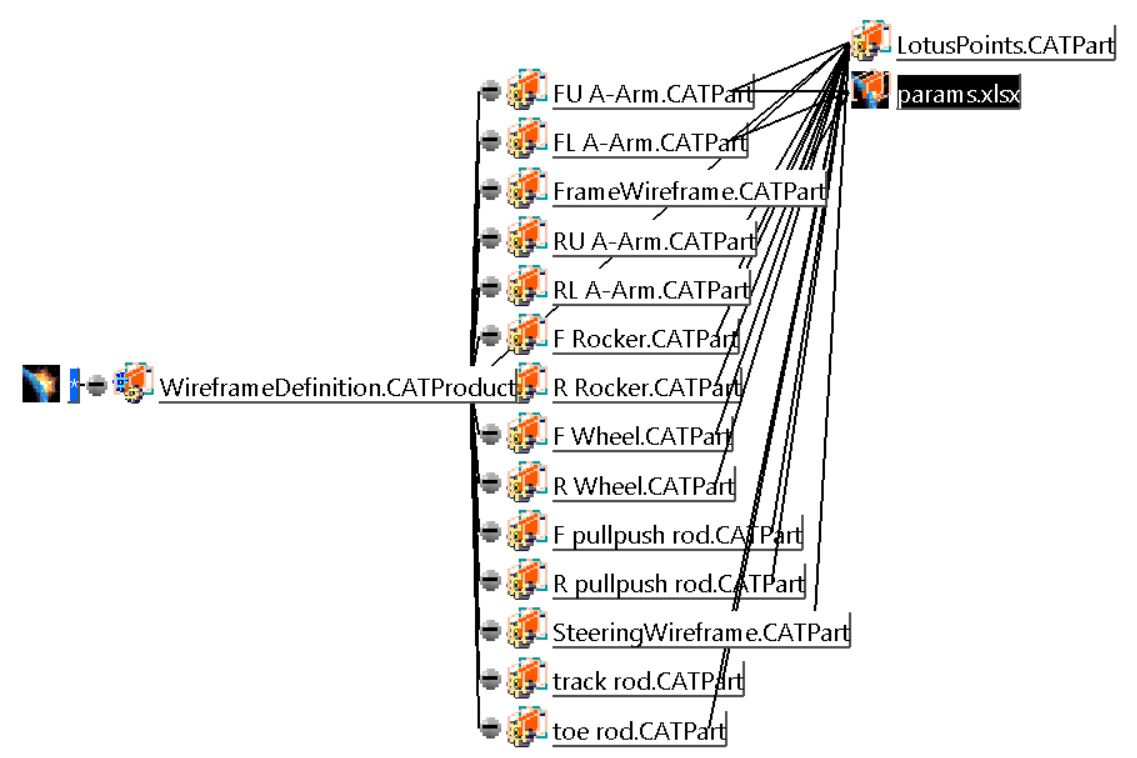
\includegraphics[height=9cm]{img/Desk_wireframe_definition.JPG}
    \caption{Capture du \textit{Bureau} de \texttt{Wireframe\_Definition.CATProduct}, montrant une structure similaire à la Figure \ref{fig:idea}}
    \label{fig:desk_wireframe_definition}
\end{figure}

% exemple de filaire type : triangles
\par Nous remarquons que dans cette étape, l'utilisateur peut définir une orientation personnalisée des repères des pièces. Cela est très utile en phase de conception détaillé afin d'avoir des produits bien faits par rapport aux directions principales du véhicule. En effet, les axes du repère Lotus sont associés à différents grandeurs caractéristiques de la dynamique du véhicule et il est par conséquent impératif que les assemblages soient bien orientés.

\subsection{Création des produits pour la conception détaillée} % ----------------

\par Dans un deuxième temps, on s'occupe de la création des fichiers pour la conception détaillée des pièces. Pour ce faire, on place, à la racine de chacun de ces produits, la pièce filaire correspondante et on la fixe avec une contrainte de fixation. Au fur et au mesure que l'on ajoute des pièces dans les produits, nous conseillons de suivre les règles suivantes:
\begin{itemize}
    \item tout positionnement de pièce à l'intérieur d'un produit de conception détaillée doit se faire par rapport à la pièce filaire à la racine du produit
    \item ranger les contraintes de chaque pièce dans un sous-dossier et cacher l'affichage graphique des contraintes 
\end{itemize}{}
\par Tout le long de la conception détaillée, on peut définir un fichier de paramètres de conception \texttt{params.xlsx} qui permettra à l'utilisateur de stocker de façon méthodique tous les paramètres inter-corrélés à l'intérieur des différents produits. Il s'agit de paramètres comme l'espacement des basculeurs ou le décalages des tubes des triangles par rapport au centre de la rotule : ces valeurs ont la caractéristique de changer très souvent pendant la période de conception du véhicule. L'exemple d'un triangle de suspension est présenté en Fig. \ref{fig:assemblage_tri}.

\begin{figure}
    \centering
    \begin{subfigure}{.5\textwidth}
        \centering
        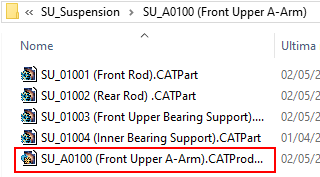
\includegraphics[width=\textwidth]{img/tria_file.png}
        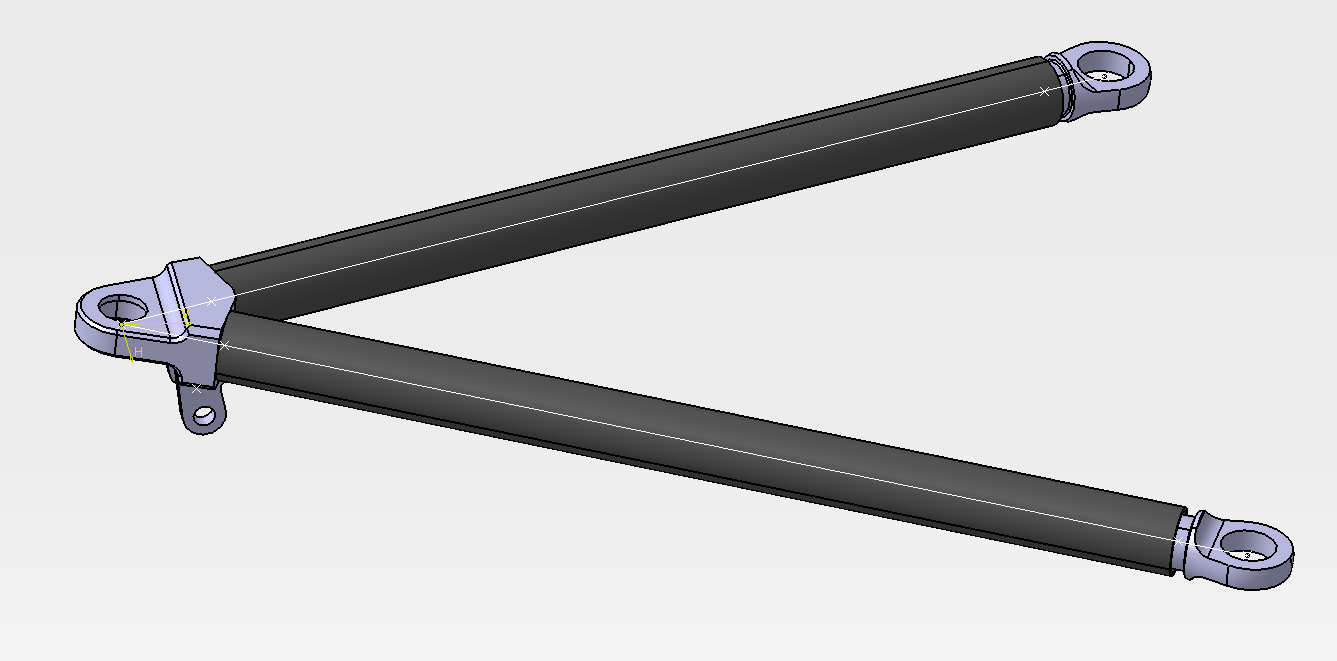
\includegraphics[width=\textwidth]{img/tria_screen.png}
    \end{subfigure}{}
    \begin{subfigure}{.25\textwidth}
        \centering
        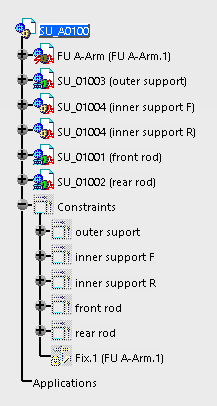
\includegraphics[width=\textwidth]{img/tria_tree.png}
    \end{subfigure}{}
    \caption{Capture d'écran du produit pour la conception détaillée du triangle avant haut gauche}
    \label{fig:assemblage_tri}
\end{figure} % image triangle détaillée

\subsection{Création d'un assemblage global pour la Liaison au Sol} % -----------------

\par Enfin, nous ajoutons les produits de conception détaillée à l'intérieur d'un assemblage général pour la totalité du système de Liaison au Sol du véhicule (Fig. \ref{fig:assemblage_las}). Pour ce faire, on place en fixation globale le produit détaillé du châssis et on accroche graduellement tous les produits détaillés.

% explication des liaisons paramétrées pour l'étude des collisions
\par Afin de pouvoir étudier le mouvement et les collisions éventuelles entre les différentes organes du véhicule, certaines  liaisons peuvent être paramétrées au niveau de l'assemblage \texttt{Suspension.CATProduct} : c'est l'exemple du débattement de l'amortisseur (paramètre \texttt{FL offset}) dans l'arbre du produit.

% explication des système e mesure pour controler les dimension critiques 
De même, certaines grandeurs caractéristiques (comme par exemple la voie et empattement) pourront être implémentées comme applications de type \textit{mesure} dans l'arbre de ce produit global afin de pouvoir surveiller leur valeur tout le long de la conception. 

\begin{figure}
    \centering
    \begin{subfigure}{.5\textwidth}
        \centering
        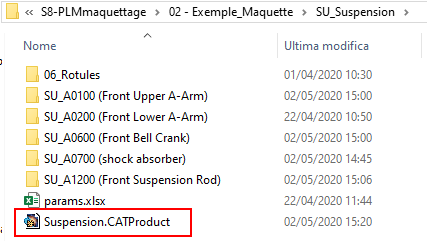
\includegraphics[width=\textwidth]{img/susp_file.png}
        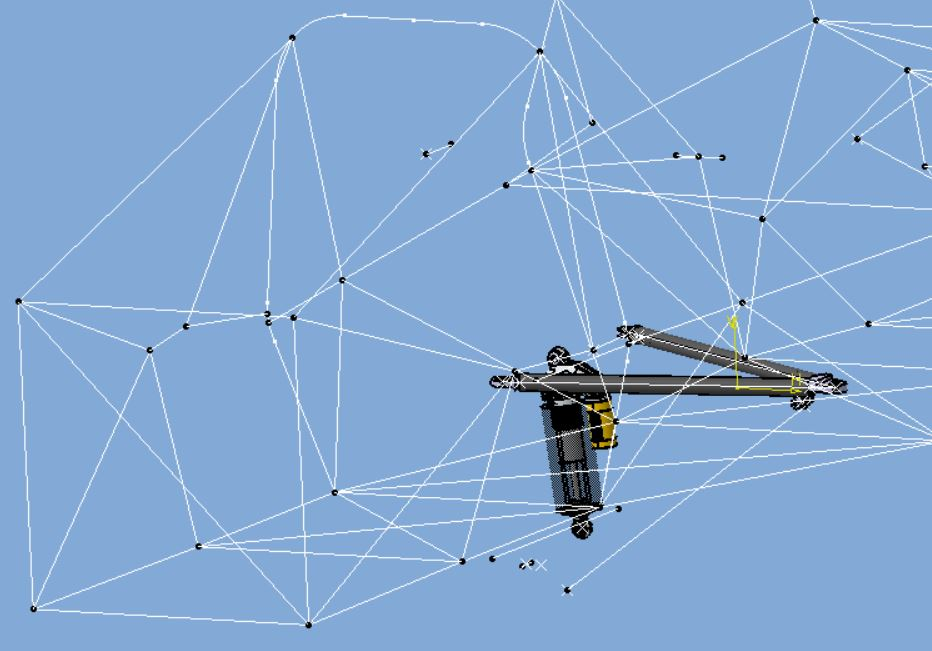
\includegraphics[width=\textwidth]{img/susp_screen.JPG}
    \end{subfigure}{}
    \begin{subfigure}{.25\textwidth}
        \centering
        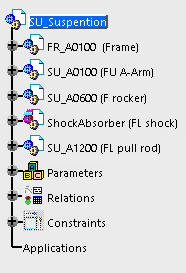
\includegraphics[width=\textwidth]{img/susp_tree.png}
    \end{subfigure}{}
    \caption{Capture d'écran de l'Assemblage LAS qui est mis à jour par la macro}
    \label{fig:assemblage_las}
\end{figure} % image suspension 

\subsection{Une proposition pour l'assemblage châssis} %-------------------------

\par Afin de démontrer la versatilité de l'architecture choisie, il est également possible d'insérer dans des assemblages d'autres sous-systèmes, certains filaires de la LAS. 
En effet, un véhicule comprend de nombreuses interactions, et la prise en compte de ces interfaces fonctionnelles est primordiale.

\par Nous proposons donc le placement du filaire des triangles de suspension et de la colonne de direction dans celui du châssis. Ces filaires seront mis à jour par la macro.

\subsection{Mise en application}

Voici les étapes à suivre pour tester la Macro, un exemple est donné en Fig. \ref{fig:maj_assy}
\begin{enumerate}
    \item Installez la macro comme spécifié dans le guide d'installation, présent dans la section \ref{install_macro}.
    \item Lancez la macro comme indiqué dans ce même guide.
    \item Sélectionnez le fichier Lotus \texttt{Test1.dat}, rangé dans le dossier \textit{04 - Tests}
    \item Sélectionnez le produit \texttt{WireframeDefinition}, dans le dossier \textit{02 - Exemple\_Maquette > wireframe}
    \item Ajoutez les produits que vous souhaitez mettre à jour dans le dossier \textit{02 - Exemple\_Maquette}, par exemple le fichier \texttt{SU\_A0100 (Front Uper A-Arm).CATProduct}
    \item Mettez à jour. Vous aurez normalement des messages d'informations sur le contenu de la mise à jour.
    \item Fermez la macro et observez l'assemblage \texttt{Suspension}
    \item Relancez la macro et répétez les étapes précédentes la concernant, en choisissant cette fois ci le fichier \texttt{Test2.dat} dans le dossier \textit{04 - Tests}. Vous devriez voir notamment que vos choix précédents ont été mis en mémoire par la macro et que vous n'aurez pas à sélectionner à nouveau \texttt{WireframeDefinition.CATProduct} et \texttt{Suspension.CATProduct}.
    \item Mettez à jour et observez l'assemblage \texttt{Suspension}. Vous pourrez noter que l'architecture a bel et bien été mis à jour.
\end{enumerate}

\begin{figure}
    \centering
    \begin{subfigure}{.35\textwidth}
        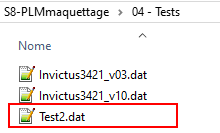
\includegraphics[width=.8\textwidth]{img/maj_file1.png}
        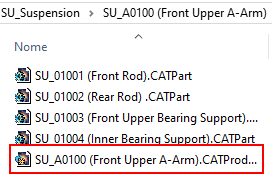
\includegraphics[width=\textwidth]{img/maj_file3.png}
    \end{subfigure}{}
    \begin{subfigure}{.3\textwidth}
        \centering
        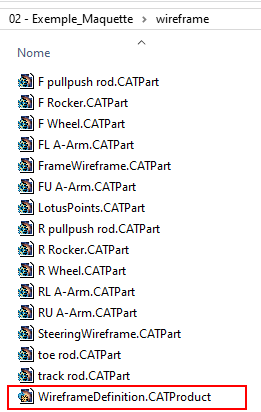
\includegraphics[width=\textwidth]{img/maj_file2.png}
    \end{subfigure}{}
    \begin{subfigure}{.3\textwidth}
        \centering
        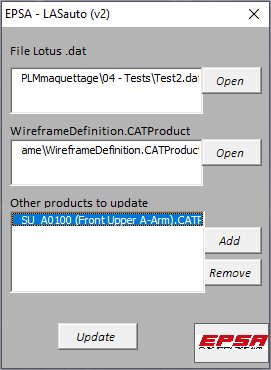
\includegraphics[width=\textwidth]{img/maj_screen.png}
    \end{subfigure}{}
    \caption{exemple de test de la macro}
    \label{fig:maj_assy}
\end{figure} % capture d'écran mise en application 